\documentclass[10pt,twocolumn]{article}

% ── Packages ──────────────────────────────────────────────────────────────
\usepackage[margin=1in]{geometry}
\usepackage{times}
\usepackage{microtype}
\usepackage{hyperref}
\usepackage{graphicx}
\usepackage{amsmath}
\usepackage{amssymb}
\usepackage{booktabs}
\usepackage{tabularx}
\usepackage{multirow}
\usepackage{listings}
\usepackage{xcolor}
\usepackage{enumitem}
\usepackage{tikz}
\usepackage{pgfplots}
\usepackage{caption}
\usepackage{subcaption}
\usepackage{abstract}
\usepackage{titlesec}
\usepackage{fancyhdr}
\usepackage{cite}
\usepackage{url}
\usepackage{balance}
\usepackage{array}
\usepackage{mdframed}

\pgfplotsset{compat=1.18}
\usetikzlibrary{arrows.meta, shapes, positioning, fit, backgrounds, calc}

% ── Colors ────────────────────────────────────────────────────────────────
\definecolor{codeblue}{RGB}{30,90,160}
\definecolor{codegray}{RGB}{100,100,100}
\definecolor{codegreen}{RGB}{30,120,60}
\definecolor{codebg}{RGB}{248,248,252}
\definecolor{accentblue}{RGB}{31,78,121}

% ── Code listing style ────────────────────────────────────────────────────
\lstset{
  backgroundcolor=\color{codebg},
  basicstyle=\ttfamily\scriptsize,
  breaklines=true,
  captionpos=b,
  commentstyle=\color{codegreen},
  keywordstyle=\color{codeblue}\bfseries,
  stringstyle=\color{codegray},
  frame=single,
  framerule=0.4pt,
  rulecolor=\color{gray!40},
  xleftmargin=6pt,
  xrightmargin=6pt,
  aboveskip=6pt,
  belowskip=6pt,
  numbers=none,
  showstringspaces=false,
  tabsize=2,
}

% ── Section formatting ────────────────────────────────────────────────────
\titleformat{\section}{\large\bfseries\color{accentblue}}{{\thesection}}{0.5em}{}
\titleformat{\subsection}{\normalsize\bfseries}{{\thesubsection}}{0.5em}{}
\titleformat{\subsubsection}{\normalsize\itshape}{{\thesubsubsection}}{0.5em}{}

% ── Header / footer ───────────────────────────────────────────────────────
\pagestyle{fancy}
\fancyhf{}
\fancyhead[L]{\small\textit{Generative Node Orchestration Technology (GNOT)}}
\fancyhead[R]{\small\textit{Viet Tran, 2026}}
\fancyfoot[C]{\thepage}
\renewcommand{\headrulewidth}{0.4pt}

% ── Hyperref setup ────────────────────────────────────────────────────────
\hypersetup{
  colorlinks=true,
  linkcolor=accentblue,
  citecolor=codegreen,
  urlcolor=codeblue,
  pdftitle={GNOT: Generative Node Orchestration Technology — A Minimal-Seed Architecture for LLM-Native Distributed Execution},
  pdfauthor={Viet Tran},
}

% ── Abstract style ────────────────────────────────────────────────────────
\renewcommand{\abstractnamefont}{\normalfont\bfseries}
\renewcommand{\abstracttextfont}{\normalfont\small}

% ═══════════════════════════════════════════════════════════════════════════
\begin{document}

% ── Title block ───────────────────────────────────────────────────────────
\title{%
  \textbf{GNOT: Generative Node Orchestration Technology}\\[4pt]
  \large A Minimal-Seed Architecture for LLM-Native Distributed Execution
}

\author{%
  \textbf{Viet Tran} \\
  \small gnot.io \\
  \small \href{mailto:viettran@gnot.io}{viettran@gnot.io}
}

\date{March 2026}

\maketitle
\thispagestyle{fancy}

% ── Abstract ──────────────────────────────────────────────────────────────
\begin{abstract}
We present \textbf{Generative Node Orchestration Technology (GNOT)}, a
distributed execution mesh designed to be orchestrated natively by large
language models. GNOT exposes a uniform \texttt{POST /action} interface
across all nodes: an LLM---whether a cloud-hosted assistant such as
Claude, a self-hosted model, or any tool-calling-capable system---can
drive the full mesh by issuing structured action requests against this
single endpoint, with no framework SDK, no workflow DSL, and no
pre-written automation code.

The system bootstraps from a single \emph{seed node} carrying three
irreducible primitive capabilities---\texttt{read\_file},
\texttt{write\_file}, and \texttt{execute\_command}---and propagates
itself across any reachable machine over HTTP. Complex multi-step
workflows are expressed as free-text intents, decomposed autonomously
through a ReAct~\cite{react2022} agent loop, and executed across nodes
that may span multiple NAT boundaries. Nodes optionally host a
configurable LLM provider, activating a \texttt{POST /intent} endpoint
for embedded orchestration; however, this is an additive capability---
the external LLM model is the primary and production-validated
interaction mode.

Key architectural contributions include: (1) a \emph{minimal-seed
bootstrap model} in which the LLM provisions new compute nodes using
only the three primitives; (2) a \emph{BGP-inspired route advertisement
protocol} enabling multi-hop NAT traversal without topology prior
knowledge; (3) a \emph{transparent push/pull delivery abstraction}
that makes network topology invisible to the LLM caller; (4) a
\emph{per-session AES-256-GCM credential system} with key derivation
scoped to each session; and (5) a \emph{lazy evaluation pattern}
applied uniformly to staleness detection, job timeouts, and file expiry.
GNOT has been deployed in production across four heterogeneous Linux
nodes spanning two NAT layers, with validated use cases including
cross-network database migration, Telegram-based CRM integration,
autonomous software development, and AI-driven content publishing.
\end{abstract}

\noindent\textbf{Keywords:} distributed systems, large language models, orchestration,
autonomous agents, ReAct, NAT traversal, BGP routing, edge computing

\vspace{4pt}
\noindent\textbf{ACM CCS:} Networks $\to$ Network architectures;
Computing methodologies $\to$ Intelligent agents

\section{Introduction}

The emergence of instruction-following large language models has created
a new class of automation systems variously called ``AI agents,''
``LLM orchestrators,'' and ``agentic pipelines.''~\cite{langchain2023,
react2022}. The dominant architectural pattern in these systems is a
\emph{wrapper model}: the LLM is given a curated set of named
tools---API endpoints, function schemas---that it invokes to interact
with the external world. Tools are authored by engineers, schemas are
static, and the LLM is fundamentally a consumer of a pre-provisioned
toolset.

This architecture works well for narrow task domains but exhibits three
structural limitations at scale:

\begin{itemize}[noitemsep, leftmargin=12pt]
  \item \textbf{Static capability boundary.} New capabilities require
    engineering effort to define and expose as tools. The LLM cannot
    extend its own toolset at runtime.
  \item \textbf{Topology blindness.} Tools abstract away network
    topology, making it impossible for the LLM to reason about which
    physical machine executes which task---relevant for latency, data
    locality, and resource-constrained deployments.
  \item \textbf{No NAT awareness.} Real enterprise and edge deployments
    routinely place compute behind NAT layers. Existing frameworks
    assume reachability and provide no first-class mechanism for NAT
    traversal.
\end{itemize}

GNOT addresses these limitations through a different framing: rather
than asking \emph{which tools should we give the LLM}, GNOT asks
\emph{what interface should the infrastructure expose so that any LLM
can orchestrate it natively}. The answer is a uniform
\texttt{POST /action} endpoint, a self-describing capability tree at
\texttt{GET /capabilities}, and a single generic \texttt{mesh\_action}
tool schema---sufficient for any tool-calling-capable LLM to discover
and operate the full mesh without SDK integration, workflow
configuration, or pre-written automation code.

This design has a practical consequence that distinguishes GNOT from
embedded-agent frameworks: \emph{the orchestrating LLM need not run
inside the infrastructure at all}. In production, GNOT is primarily
operated via Claude through its web interface---a frontier model with
a rich capability surface including vision input, voice interaction,
sandboxed code execution, and tool use across long contexts. A
subscription-based access model is substantially more cost-efficient
than per-token API billing for sustained automation workloads.
Critically, the mesh interface is stable while the orchestrating model
improves continuously, without any changes to node configuration or
action code.

Node-local LLM orchestration is an \emph{additive} capability: when a
node is configured with an LLM provider (cloud API or local inference
server), it activates a \texttt{POST /intent} endpoint that runs the
ReAct loop internally. This enables embedded agents, offline-capable
nodes, and per-node autonomous orchestration---complementing rather
than replacing the external model pattern.

The insight driving the bootstrap model is that three primitive
capabilities suffice to provision any computational environment: if a
machine can read files, write files, and execute shell commands, then
\emph{any} software can be installed, any configuration can be written,
and any process can be started. An LLM reasoning over these three
primitives becomes both the provisioning layer and the orchestration
layer simultaneously, without requiring any infrastructure pre-existing
beyond a running GNOT node.

The remainder of this paper is organized as follows.
Section~\ref{sec:background} reviews related work.
Section~\ref{sec:arch} presents the GNOT architecture.
Section~\ref{sec:routing} describes the routing engine and BGP-inspired
route advertisement. Section~\ref{sec:agent} covers the ReAct agent
loop and intent handling. Section~\ref{sec:security} discusses the
security model. Section~\ref{sec:bootstrap} explains self-bootstrapping.
Section~\ref{sec:deployment} describes the production deployment and
validated use cases. Section~\ref{sec:discussion} discusses design
decisions and limitations. Section~\ref{sec:conclusion} concludes.

\section{Background and Related Work}
\label{sec:background}

\subsection{LLM Orchestration Frameworks}

\textbf{LangChain}~\cite{langchain2023} is the most widely adopted
framework for building LLM-powered applications. Its agent abstraction
gives the LLM access to a registered set of tools---Python functions
with typed signatures---that it invokes to interact with the external
world. Tools are statically defined at application startup; the LLM
cannot extend its own toolset at runtime. More fundamentally, LangChain
does not address multi-machine execution: all tool calls execute within
a single process on a single host.

A growing ecosystem of agent frameworks has emerged around this same
architectural pattern---including multi-agent conversation frameworks
and role-based crew systems---sharing the same structural
limitation: the LLM is a client of pre-provisioned infrastructure,
not the infrastructure itself. Distribution across machines, NAT
traversal, and runtime self-provisioning are not first-class concerns
in any of these systems.

GNOT differs in one fundamental respect: the LLM \emph{is} the control
plane. It generates routing decisions, provisions new nodes, and
composes cross-machine workflows using the same three primitives it was
given at boot---without any static tool registration or external
orchestration layer.

\subsection{ReAct: Reasoning and Acting}

Yao et al.~\cite{react2022} introduced ReAct, a prompting strategy that
interleaves reasoning traces (\emph{Thought}) with action invocations
(\emph{Act}) and environment observations (\emph{Obs}) in an alternating
loop. The pattern allows an LLM to decompose multi-step problems, course-correct
on unexpected results, and produce a final answer only when it
has sufficient information.

GNOT adopts ReAct as the execution model of its \texttt{IntentHandler}.
The key extension over the original formulation is the action
target: where Yao et al.\ dispatch to a local function registry,
GNOT dispatches to a distributed execution mesh that may span multiple
machines across multiple NAT boundaries. The LLM's reasoning trace
therefore includes implicit decisions about \emph{where} to execute,
not only \emph{what} to execute.

\subsection{BGP and Application-Layer Routing}

The Border Gateway Protocol (BGP)~\cite{rekhter1995bgp} solves
inter-domain routing on the internet. Its central abstraction is
\emph{next-hop forwarding with route advertisement}: each autonomous
system announces the IP prefixes it can reach to its neighbors, which
propagate the announcement further. A router needs to know only its
immediate next hop toward a destination---not the full path.

GNOT maps this abstraction to the application layer. Each intermediate
mesh node advertises the sub-nodes reachable through it; the gateway
installs these routes with a next-hop pointer. The result is that a
request for a deeply nested node traverses the mesh correctly without
any node needing global topology knowledge. Section~\ref{sec:bgp}
describes the protocol in detail.

\section{System Architecture}
\label{sec:arch}

\subsection{Design Principles}

GNOT is founded on five principles:

\begin{enumerate}[noitemsep, leftmargin=14pt]
  \item \textbf{Maximal minimalism at origin.} The seed node carries
    exactly three capabilities. Everything else emerges at runtime.
  \item \textbf{LLM-native interface.} The mesh exposes a uniform,
    self-describing interface (\texttt{POST /action},
    \texttt{GET /capabilities}, \texttt{mesh\_action} tool schema)
    designed so that any tool-calling-capable LLM can orchestrate it
    natively---without SDK wrappers, static tool registration, or
    workflow configuration code.
  \item \textbf{Transparent delivery.} Whether execution is local,
    synchronous remote (push), or asynchronous queued (pull), the
    calling interface is identical: \texttt{POST /action} returning
    either an inline result or a \texttt{job\_id} for polling.
  \item \textbf{Composition over configuration.} No workflow DSL, no
    DAG executor. The LLM composes multi-step workflows through
    sequential tool calls.
  \item \textbf{LLM flexibility.} The mesh does not mandate where the
    orchestrating LLM runs. An external LLM---cloud-hosted, local, or
    subscription-accessed---is the primary and production-validated
    mode. A node-local LLM (activated via \texttt{llm\_provider}
    configuration) is an additive option for embedded or
    offline-capable deployments. Both interact with the mesh through
    the same routing layer.
\end{enumerate}

\subsection{System Architecture Overview}

Figure~\ref{fig:arch} presents the complete GNOT architecture. A node
is composed of three concentric layers: the \emph{API layer} that
receives all inbound requests, the \emph{runtime layer} that implements
routing, job management, session state, and credential storage, and the
\emph{execution layer} that runs action code. Nodes connect to each
other exclusively through their API layers; internal components are
never exposed directly.

\begin{figure*}[ht]
\centering
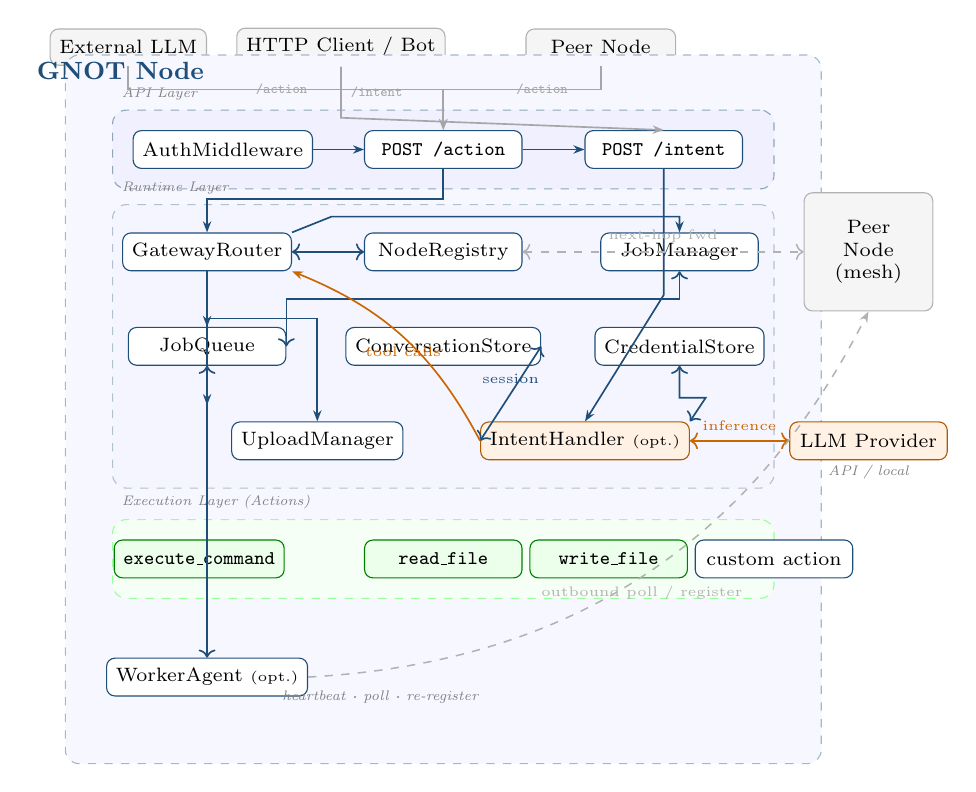
\begin{tikzpicture}[
  every node/.style={font=\scriptsize},
  layer/.style={draw, rounded corners=5pt, dashed, inner sep=6pt},
  comp/.style={draw, rounded corners=3pt, fill=white, draw=accentblue,
               minimum width=2.0cm, minimum height=0.48cm, text centered},
  llmcomp/.style={comp, fill=orange!10, draw=orange!70!black},
  seedcomp/.style={comp, fill=green!8, draw=green!50!black},
  extbox/.style={draw, rounded corners=3pt, fill=gray!8, draw=gray!60,
                 minimum width=1.9cm, minimum height=0.46cm, text centered},
  arr/.style={-{Stealth[length=4pt]}, line width=0.6pt, accentblue},
  garr/.style={-{Stealth[length=4pt]}, line width=0.6pt, gray!70},
  darr/.style={-{Stealth[length=4pt]}, dashed, line width=0.55pt, gray!60},
  larr/.style={-{Stealth[length=4pt]}, line width=0.6pt, orange!80!black},
  lbl/.style={font=\tiny, midway},
  slbl/.style={font=\tiny\itshape, text=gray},
]

%% ── EXTERNAL CALLERS (top) ────────────────────────────────────────────
\node[extbox] (extllm)  at (-4.0, 9.4) {External LLM};
\node[extbox] (httpbot) at (-1.3, 9.4) {HTTP Client / Bot};
\node[extbox] (peerint) at ( 2.0, 9.4) {Peer Node};

%% ── NODE BOUNDARY ─────────────────────────────────────────────────────
\begin{scope}
\node[layer, fill=blue!3, draw=accentblue!40,
      minimum width=9.6cm, minimum height=9.0cm]
  (nodeborder) at (0, 4.8) {};
\node[font=\small\bfseries, text=accentblue] at (-4.1, 9.1) {GNOT Node};
\end{scope}

%% ── LAYER 1: API ──────────────────────────────────────────────────────
\node[layer, fill=blue!6, draw=accentblue!50,
      minimum width=8.4cm, minimum height=1.0cm]
  (apilayer) at (0, 8.1) {};
\node[slbl, above right] at (apilayer.north west) {API Layer};

\node[comp] (authm)   at (-2.8, 8.1) {AuthMiddleware};
\node[comp] (aaction) at ( 0.0, 8.1) {\texttt{POST /action}};
\node[comp] (aintent) at ( 2.8, 8.1) {\texttt{POST /intent}};

%% ── LAYER 2: RUNTIME ──────────────────────────────────────────────────
\node[layer, fill=blue!4, draw=accentblue!35,
      minimum width=8.4cm, minimum height=3.6cm]
  (rtlayer) at (0, 5.6) {};
\node[slbl, above right] at (rtlayer.north west) {Runtime Layer};

\node[comp]    (router)   at (-3.0, 6.8) {GatewayRouter};
\node[comp]    (registry) at ( 0.0, 6.8) {NodeRegistry};
\node[comp]    (jobmgr)   at ( 3.0, 6.8) {JobManager};

\node[comp]    (jobq)     at (-3.0, 5.6) {JobQueue};
\node[comp]    (convst)   at ( 0.0, 5.6) {ConversationStore};
\node[comp]    (credst)   at ( 3.0, 5.6) {CredentialStore};

\node[comp]    (uploadm)  at (-1.6, 4.4) {UploadManager};
\node[llmcomp] (intenth)  at ( 1.8, 4.4) {IntentHandler \tiny(opt.)};

%% ── LLM PROVIDER ──────────────────────────────────────────────────────
\node[llmcomp] (llmprov) at (5.4, 4.4) {LLM Provider};
\node[slbl]    at (5.4,  4.0)          {API / local};

%% ── LAYER 3: EXECUTION ────────────────────────────────────────────────
\node[layer, fill=green!4, draw=green!40,
      minimum width=8.4cm, minimum height=1.0cm]
  (exlayer) at (0, 2.9) {};
\node[slbl, above right] at (exlayer.north west) {Execution Layer (Actions)};

\node[seedcomp] (seed1) at (-3.1, 2.9) {\texttt{execute\_command}};
\node[seedcomp] (seed2) at ( 0.0, 2.9) {\texttt{read\_file}};
\node[seedcomp] (seed3) at ( 2.1, 2.9) {\texttt{write\_file}};
\node[comp]     (plugn) at ( 4.2, 2.9) {custom action};

%% ── WORKER AGENT ──────────────────────────────────────────────────────
\node[comp] (worker) at (-3.0, 1.4) {WorkerAgent \tiny(opt.)};
\node[slbl] at (-0.8, 1.15)         {heartbeat · poll · re-register};

%% ── PEER NODE (right) ─────────────────────────────────────────────────
\node[extbox, minimum height=1.5cm, minimum width=1.5cm,
      text width=1.4cm, text centered]
  (peernode) at (5.4, 6.8) {Peer\\Node\\(mesh)};

%% ═════════════════════════════════════════════════════════════════════
%% ARROWS
%% ═════════════════════════════════════════════════════════════════════

%% External callers → API layer
\draw[garr] (extllm.south)  -- ++(0,-0.3) -| node[left, lbl, pos=0.3]{\texttt{/action}} (aaction.north);
\draw[garr] (httpbot.south) -- node[right, lbl]{\texttt{/intent}} ++(0,-0.65) -- (aintent.north);
\draw[garr] (peerint.south) -- ++(0,-0.3) -| node[right, lbl, pos=0.3]{\texttt{/action}} (aaction.north);

%% Auth gates all
\draw[arr] (authm.east) -- (aaction.west);
\draw[arr] (aaction.east) -- (aintent.west);

%% /action → GatewayRouter
\draw[arr] (aaction.south) -- ++(0,-0.38) -| (router.north);

%% /intent → IntentHandler
\draw[arr] (aintent.south) -- ++(0,-1.6) -- (intenth.north);

%% GatewayRouter ↔ NodeRegistry
\draw[arr, <->] (router.east) -- (registry.west);

%% GatewayRouter → JobManager
\draw[arr] (router.north east) -- ++(0.5,0.2) -| (jobmgr.north);

%% GatewayRouter → JobQueue
\draw[arr] (router.south) -- (jobq.north);

%% JobManager ↔ JobQueue
\draw[arr, <->] (jobmgr.south) -- ++(0,-0.35) -| (jobq.east);

%% GatewayRouter → Execution layer
\draw[arr] (router.south) -- ++(0,-1.7);

%% IntentHandler ↔ ConversationStore
\draw[arr, <->] (intenth.west) -- node[above, lbl]{session} (convst.east);

%% IntentHandler ↔ CredentialStore
\draw[arr, <->] (intenth.north east) -- ++(0.2,0.3) -| (credst.south);

%% IntentHandler → GatewayRouter (tool calls)
\draw[larr, bend right=20] (intenth.west) to
  node[below, lbl, text=orange!80!black]{tool calls} (router.south east);

%% IntentHandler ↔ LLM Provider
\draw[larr, <->] (intenth.east) --
  node[above, lbl, text=orange!80!black]{inference} (llmprov.west);

%% UploadManager ← Router
\draw[arr] (router.south) -- ++(0,-0.6) -| (uploadm.north);

%% WorkerAgent ↔ JobQueue
\draw[arr, <->] (worker.north) -- (jobq.south);

%% WorkerAgent → Peer gateway (outbound)
\draw[darr, bend right=30] (worker.east) to
  node[below, lbl]{outbound poll / register} (peernode.south);

%% NodeRegistry ↔ Peer Node (next-hop forwarding)
\draw[darr, <->] (registry.east) --
  node[above, lbl]{next-hop fwd} (peernode.west);

\end{tikzpicture}
\caption{GNOT system architecture overview. Three layers handle all
request processing: the API layer (AuthMiddleware, endpoints), the
Runtime layer (routing, job management, session and credential stores),
and the Execution layer (seed actions and custom plugins). The
\texttt{IntentHandler} and LLM Provider (orange) are optional,
activated only when \texttt{llm\_provider} is configured. The
\texttt{WorkerAgent} (optional) enables pull-mode operation for nodes
behind NAT. Dashed arrows indicate optional or asynchronous flows.}
\label{fig:arch}
\end{figure*}

\subsection{Node Anatomy}

Every GNOT node is an HTTP service running on a Linux machine. Its
filesystem structure is minimal:

\begin{lstlisting}[language=bash, caption={Node directory structure}]
/opt/mesh/<node-id>/
  node.yaml          # configuration
  actions/
    execute_command.py
    execute_command.schema.json
    read_file.py
    read_file.schema.json
    write_file.py
    write_file.schema.json
    <custom_action>.py          # optional
    <custom_action>.schema.json # optional
\end{lstlisting}

The runtime (\texttt{node\_runtime.py} and the \texttt{runtime/} package)
is shared across all nodes on a machine and installed once. Nodes are
differentiated only by their \texttt{node.yaml} configuration and their
\texttt{actions/} directory contents.

\subsection{Node Operating Modes}

A node operates in one or more modes simultaneously, determined solely
by its configuration (Table~\ref{tab:modes}).

\begin{table}[h]
\centering
\caption{Node operating modes}
\label{tab:modes}
\small
\begin{tabular}{@{}lp{5.2cm}@{}}
\toprule
\textbf{Mode} & \textbf{Condition and Role} \\
\midrule
Standalone & No peers configured. Executes actions locally only. \\
Gateway & \texttt{trusted\_nodes} configured. Accepts worker registrations, routes requests, hosts IntentHandler. \\
Worker & \texttt{gateway\_node\_id} + \texttt{gateway\_address} set. Polls gateway, executes jobs. \\
Gateway+Worker & Both conditions. Intermediate node: routes to sub-nodes and is itself a worker. \\
\bottomrule
\end{tabular}
\end{table}

\subsection{Topology Overview}

Figure~\ref{fig:topology} illustrates a representative GNOT deployment.
A gateway node is publicly reachable (via Cloudflare Tunnel or direct IP)
and accepts requests from external callers---web interfaces, Telegram
bots, or HTTP clients. Worker nodes behind one or more NAT layers
connect outward to the gateway; they never receive inbound connections.

\subsection{LLM Interaction Model}
\label{sec:dual}

GNOT is designed so that the LLM orchestrator is \emph{decoupled from
the node runtime}. Every node exposes \texttt{POST /action}
unconditionally; \texttt{POST /intent} is an optional endpoint,
activated only when an \texttt{llm\_provider} is configured. This
yields two complementary interaction patterns
(Figure~\ref{fig:dual}):

\textbf{Pattern A --- External LLM (primary).}
An LLM operating outside the mesh acts as the orchestrator. The user
provides the LLM with the mesh capability description from
\texttt{GET /capabilities} and the \texttt{mesh\_action} tool schema.
The LLM then drives the mesh directly via \texttt{POST /action},
carrying \texttt{target\_node\_id}, action name, and parameters per
request. The node runtime executes, routes, or queues each request with
no LLM involvement on any node.

This is the primary and production-validated pattern. In the reference
deployment, Claude---accessed via its web interface---serves as the
orchestrator. This approach offers several practical advantages over
embedding an LLM inside the infrastructure:

\begin{itemize}[noitemsep, leftmargin=12pt]
  \item \textbf{Richer capability surface.} A frontier model accessed
    through a full-featured interface provides vision input, voice
    interaction, sandboxed code execution, extended context windows,
    and continuous model improvements---all without changes to node
    configuration.
  \item \textbf{Cost efficiency.} Subscription-based access to a
    frontier model is substantially more economical than per-token API
    billing for sustained multi-step automation workloads.
  \item \textbf{Zero inference overhead on mesh nodes.} Execution nodes
    remain lightweight and resource-predictable; no GPU or model
    serving infrastructure is required anywhere in the mesh.
\end{itemize}

\textbf{Pattern B --- Node-local LLM (additive).}
When a node is configured with an \texttt{llm\_provider} (external API
or local inference server such as Ollama or vLLM), it activates the
\texttt{IntentHandler} and exposes \texttt{POST /intent}. A caller
submits a free-text prompt; the node's LLM decomposes it into
\texttt{mesh\_action} tool calls, dispatches them through the same
\texttt{GatewayRouter} as Pattern A, and returns a synthesized
natural-language response. This pattern suits use cases requiring
low-latency embedded agents, air-gapped or offline deployments, or
per-node autonomous decision making.

\begin{figure}[h]
\centering
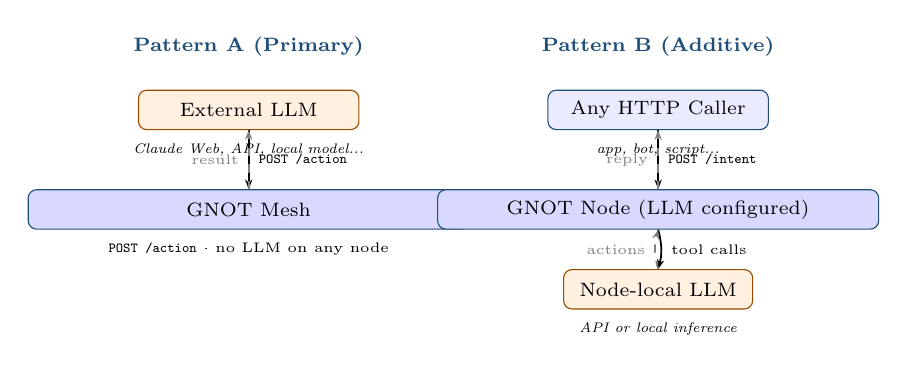
\begin{tikzpicture}[
  node distance=0.5cm and 0.8cm,
  box/.style={draw, rounded corners=3pt, font=\scriptsize,
              fill=blue!8, draw=accentblue,
              minimum width=2.8cm, minimum height=0.5cm},
  llmbox/.style={draw, rounded corners=3pt, font=\scriptsize,
              fill=orange!12, draw=orange!60!black,
              minimum width=2.8cm, minimum height=0.5cm},
  meshbox/.style={draw, rounded corners=3pt, font=\scriptsize,
              fill=blue!15, draw=accentblue,
              minimum width=5.6cm, minimum height=0.5cm},
  arr/.style={-{Stealth[length=3.5pt]}, line width=0.65pt},
  darr/.style={-{Stealth[length=3.5pt]}, dashed, gray, line width=0.65pt},
  lbl/.style={font=\tiny, midway},
]

% ── Pattern A ────────────────────────────────────────────────
\node[font=\scriptsize\bfseries, color=accentblue] (ta) at (-1.8, 0)
  {Pattern A (Primary)};

\node[llmbox, below=0.3cm of ta] (extllm)
  {External LLM};
\node[font=\tiny\itshape, below=0.05cm of extllm]
  {Claude Web, API, local model...};

\node[meshbox, below=0.75cm of extllm] (meshA)
  {GNOT Mesh};
\node[font=\tiny, below=0.05cm of meshA]
  {\texttt{POST /action} · no LLM on any node};

\draw[arr] (extllm.south) -- node[right, lbl]{\texttt{POST /action}} (meshA.north);
\draw[darr] (meshA.north) -- node[left, lbl]{result} (extllm.south);

% ── Pattern B ────────────────────────────────────────────────
\node[font=\scriptsize\bfseries, color=accentblue] (tb) at (3.4, 0)
  {Pattern B (Additive)};

\node[box, below=0.3cm of tb] (caller)
  {Any HTTP Caller};
\node[font=\tiny\itshape, below=0.05cm of caller]
  {app, bot, script...};

\node[meshbox, below=0.75cm of caller] (meshB)
  {GNOT Node (LLM configured)};

\node[llmbox, below=0.5cm of meshB, minimum width=2.4cm] (nodellm)
  {Node-local LLM};
\node[font=\tiny\itshape, below=0.05cm of nodellm]
  {API or local inference};

\draw[arr] (caller.south) -- node[right, lbl]{\texttt{POST /intent}} (meshB.north);
\draw[darr] (meshB.north) -- node[left, lbl]{reply} (caller.south);
\draw[arr, bend left=15] (meshB.south) to
  node[right, lbl]{tool calls} (nodellm.north);
\draw[darr, bend left=15] (nodellm.north) to
  node[left, lbl]{actions} (meshB.south);

\end{tikzpicture}
\caption{LLM interaction patterns. Pattern A (primary): an external LLM
orchestrates the full mesh via \texttt{POST /action}; no LLM is
required on any node. Pattern B (additive): a configured node-local LLM
processes free-text intents via \texttt{POST /intent}, dispatching the
same \texttt{mesh\_action} tool calls through the same routing layer.
Both patterns can coexist in the same deployment.}
\label{fig:dual}
\end{figure}

The two patterns are not mutually exclusive: some nodes may run
node-local LLMs for embedded processing while others operate as pure
execution nodes reachable from any external orchestrator.
The routing layer is identical in both cases.


\begin{figure}[h]
\centering
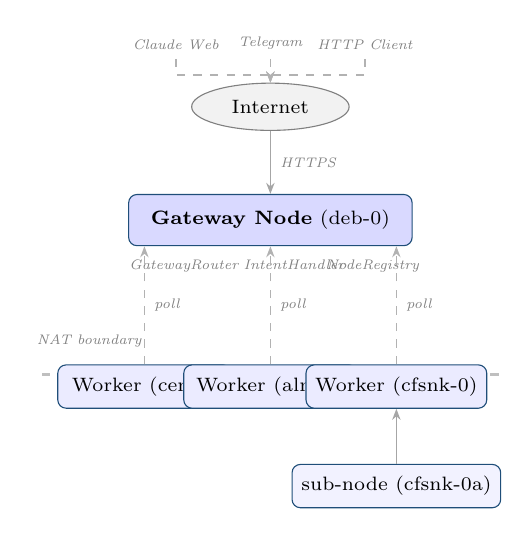
\begin{tikzpicture}[
  node distance=0.7cm and 1.0cm,
  box/.style={draw, rounded corners=3pt, font=\scriptsize,
              minimum width=2.2cm, minimum height=0.55cm,
              fill=blue!8, draw=accentblue},
  cloud/.style={draw, ellipse, font=\scriptsize,
                fill=gray!10, draw=gray, minimum width=2.0cm, minimum height=0.6cm},
  arr/.style={-{Stealth[length=4pt]}, gray!70, line width=0.6pt},
  darr/.style={-{Stealth[length=4pt]}, dashed, gray!60, line width=0.6pt},
  label/.style={font=\tiny\itshape, text=gray},
]

% Internet / external callers
\node[cloud] (internet) {Internet};

% External callers above
\node[label, above=0.3cm of internet, xshift=-1.2cm] (claude) {Claude Web};
\node[label, above=0.3cm of internet, xshift=0cm]    (tg)     {Telegram};
\node[label, above=0.3cm of internet, xshift=1.2cm]  (curl)   {HTTP Client};
\draw[darr] (claude.south) -- ++(0,-0.2) -| (internet);
\draw[darr] (tg.south) -- (internet);
\draw[darr] (curl.south) -- ++(0,-0.2) -| (internet);

% Gateway node
\node[box, below=0.8cm of internet, minimum width=3.6cm, minimum height=0.65cm,
      fill=blue!15] (gw) {\textbf{Gateway Node} (deb-0)};
\draw[arr] (internet) -- (gw) node[midway, right, label]{HTTPS};

% Components inside gateway
\node[label, below=0.05cm of gw, xshift=-1.1cm] (router_l) {GatewayRouter};
\node[label, below=0.05cm of gw, xshift=0.3cm]  (intent_l) {IntentHandler};
\node[label, below=0.05cm of gw, xshift=1.3cm]  (reg_l)    {NodeRegistry};

% NAT boundary
\node[label, below=1.0cm of gw, xshift=-2.3cm] (nat_label) {NAT boundary};
\draw[dashed, gray!50, line width=0.8pt] (-2.9,-3.4) -- (2.9,-3.4);

% Worker nodes
\node[box, below=1.5cm of gw, xshift=-1.6cm] (w1) {Worker (cen-0)};
\node[box, below=1.5cm of gw, xshift=0cm]    (w2) {Worker (alm-0)};
\node[box, below=1.5cm of gw, xshift=1.6cm]  (w3) {Worker (cfsnk-0)};

% Sub-node under cfsnk-0
\node[box, below=0.7cm of w3, minimum width=2.0cm, fill=blue!5] (sub) {\scriptsize sub-node (cfsnk-0a)};

% Pull arrows (workers poll upward)
\draw[darr] (w1.north) -- node[right, label]{poll} (gw.south -| w1.north);
\draw[darr] (w2.north) -- node[right, label]{poll} (gw.south -| w2.north);
\draw[darr] (w3.north) -- node[right, label]{poll} (gw.south -| w3.north);
\draw[arr]  (sub.north) -- (w3.south);

\end{tikzpicture}
\caption{GNOT deployment topology. Workers poll the gateway outbound (dashed arrows); the gateway never initiates connections to workers behind NAT.}
\label{fig:topology}
\end{figure}

\subsection{Principal Components}

Table~\ref{tab:components} summarizes the principal runtime components.

\begin{table}[h]
\centering
\caption{Principal GNOT components}
\label{tab:components}
\small
\begin{tabular}{@{}lp{5.0cm}@{}}
\toprule
\textbf{Component} & \textbf{Responsibility} \\
\midrule
GatewayRouter & Routes \texttt{POST /action} to correct delivery path: local / push / pull / next-hop forward. \\
NodeRegistry & Tracks trusted nodes, liveness, addresses, capabilities, and BGP next-hop entries. \\
JobManager & Maintains job state machine (\texttt{accepted} $\to$ \texttt{running} $\to$ \texttt{completed}/\texttt{failed}). \\
JobQueue & Per-node pull queue; holds jobs for workers that cannot receive inbound connections. \\
WorkerAgent & Three asyncio tasks inside each worker: registration, heartbeat, poll-execute-report. \\
IntentHandler & ReAct loop: converts free-text prompts into mesh action sequences. \\
ConversationStore & Per-session message history for multi-turn conversations. \\
CredentialStore & AES-256-GCM encrypted store for caller-supplied credentials. \\
UploadManager & Staged binary file store enabling large-file cross-NAT transfer. \\
\bottomrule
\end{tabular}
\end{table}

\subsection{Capability Discovery}
\label{sec:discovery}

Every GNOT node exposes a \texttt{GET /capabilities} endpoint that
returns the complete capability tree of the node and all nodes
reachable through it---including action specifications, parameter
schemas, caller credential requirements, liveness status, and
next-hop routing information:

\begin{lstlisting}[caption={Capability tree response (excerpt)}]
GET /capabilities
{
  "node_id": "deb-0",
  "actions": ["execute_command", "read_file", "write_file"],
  "reachable": {
    "cen-0": {
      "status":   "online",
      "next_hop": null,
      "actions":  ["execute_command", "read_file", "write_file"],
      "action_specs": {
        "execute_command": {
          "description": "Execute shell command",
          "params_schema": {
            "command": { "type": "string" },
            "timeout_seconds": { "type": "integer", "default": 60 }
          },
          "async_action": true
        }
      }
    },
    "cfsnk-0a": {
      "status":   "online",
      "next_hop": "cfsnk-0",
      "actions":  ["get_order_info"],
      "action_specs": {
        "get_order_info": {
          "caller_credentials": {
            "crm_user_token": {
              "description": "CRM API key",
              "required": true
            }
          }
        }
      }
    }
  }
}
\end{lstlisting}

The \texttt{status} field reflects a lazy staleness check at query
time (Section~\ref{sec:lazy}). The \texttt{next\_hop} field exposes
the BGP-style routing entry transparently: a caller targeting
\texttt{cfsnk-0a} need not know that \texttt{cfsnk-0} is the
intermediate node---the gateway handles forwarding automatically.

\texttt{GET /capabilities} is the primary mechanism by which an
external LLM (Model A, Section~\ref{sec:dual}) learns the mesh
topology before issuing \texttt{POST /action} calls. For Model B, the
\texttt{IntentHandler} calls this endpoint internally to generate the
dynamic system prompt at each \texttt{POST /intent} request.

A legacy \texttt{GET /skills} endpoint returns a human-readable
Markdown description of node capabilities, retained for backward
compatibility with external LLM workflows that inject skills as
freeform context rather than structured JSON.

\subsection{Observability}
\label{sec:health}

\texttt{GET /health} returns a structured summary of node state:

\begin{lstlisting}[caption={Health endpoint response}]
{
  "node_id":        "deb-0",
  "status":         "healthy",
  "uptime_seconds": 3600.5,
  "actions_loaded": 5,
  "jobs_active":    2,
  "queue_depths": {
    "cen-0":   3,
    "alm-0":   0,
    "cfsnk-0": 1
  }
}
\end{lstlisting}

The \texttt{queue\_depths} field reports unclaimed jobs per worker
node in the pull queue. This field serves three operational purposes:
detecting stuck workers (depth growing while worker is offline),
triggering scale-out decisions (depth exceeding threshold $\to$
bootstrap new worker via \texttt{execute\_command}), and general
health monitoring. At the L3 evolution level
(Section~\ref{sec:bootstrap}), an LLM observing
\texttt{queue\_depths} can autonomously decide to provision additional
worker nodes and decommission them when load subsides---closing the
self-optimization loop entirely within the mesh.

\section{Routing Engine}
\label{sec:routing}

\subsection{Request Envelope}

Every action request follows a uniform envelope:

\begin{lstlisting}[language=, caption={Action request envelope}]
{
  "target_node_id": "cfsnk-0a",
  "payload": {
    "action": "execute_command",
    "params": { "command": "df -h" }
  },
  "task_id": "task-3f8a91c2b4e1",  // auto-generated if absent
  "trace": { "hop_count": 0, "route_path": [] },
  "caller_credentials": {}
}
\end{lstlisting}

The response is either synchronous (inline \texttt{output}) or
asynchronous (a \texttt{job\_id} for polling). The \emph{presence of
\texttt{job\_id}} is the sole indicator of async mode; the caller sets
no mode flag.

\subsection{GatewayRouter Decision Tree}

Every node runs a \texttt{GatewayRouter} that applies the following
decision tree on every \texttt{POST /action}:

\begin{lstlisting}[caption={Routing decision logic (pseudocode)}]
route(request):
  1. if hop_count > max_hop:       MAX_HOP_EXCEEDED
  2. if node_id in route_path:     LOOP_DETECTED
  3. if target == self:            execute_local()
  4. next_hop = registry.get_next_hop(target)
     if next_hop != target:        forward_via_next_hop()
  5. if not registry.is_trusted(target): UNTRUSTED_NODE
  6. address = registry.get_address(target)
     if not address:               pull(request)
     elif ping(target):            result = push(address, request)
       if error:                   pull(request)   // fallback
     else:                         pull(request)
\end{lstlisting}

Steps 1--2 prevent routing loops. Step 4 implements the BGP-inspired
next-hop forwarding described in Section~\ref{sec:bgp}. Step 6 provides
the transparent push/pull abstraction described in
Section~\ref{sec:pushpull}.

\subsection{BGP-Inspired Route Advertisement}
\label{sec:bgp}

A fundamental challenge in heterogeneous network deployments is that the
gateway may not have direct connectivity to all nodes. Consider a
three-layer topology:

\begin{center}
\texttt{gateway (deb-0) $\to$ node-1 $\to$ node-1a}
\end{center}

Without any route advertisement mechanism, the gateway cannot route
requests to \texttt{node-1a}: it has no entry for that node. GNOT
solves this with a protocol analogous to BGP route advertisement.

\textbf{Advertisement flow.} When \texttt{node-1a} registers with
\texttt{node-1}, it includes its action list. \texttt{node-1}'s
\texttt{WorkerAgent} then re-registers with the gateway, including
\texttt{node-1a} in its \texttt{advertise\_routes} list:

\begin{lstlisting}[caption={Re-registration with route advertisement}]
POST gateway/nodes/register {
  "node_id": "node-1",
  "actions": ["execute_command"],
  "advertise_routes": ["node-1a"],
  "capabilities": {
    "node-1a": ["execute_command", "get_order_info"]
  },
  "sub_route_specs": {
    "node-1a": { "get_order_info": { ...full spec... } }
  }
}
\end{lstlisting}

The gateway installs \texttt{node-1a} with \texttt{next\_hop = node-1}.
Subsequent requests for \texttt{node-1a} are forwarded to \texttt{node-1},
which then routes to \texttt{node-1a} directly.

\textbf{BGP analogy.} Table~\ref{tab:bgp} maps BGP concepts to their
GNOT equivalents.

\begin{table}[h]
\centering
\caption{BGP-to-GNOT concept mapping}
\label{tab:bgp}
\small
\begin{tabular}{@{}ll@{}}
\toprule
\textbf{BGP Concept} & \textbf{GNOT Equivalent} \\
\midrule
Autonomous System & Node \\
IP prefix & Node ID \\
BGP neighbor & Gateway node \\
Route advertisement & \texttt{advertise\_routes} in \texttt{POST /nodes/register} \\
Next-hop router & \texttt{next\_hop} in \texttt{NodeRegistry} entry \\
BGP UPDATE message & Periodic WorkerAgent re-registration \\
BGP WITHDRAW message & Re-registration with reduced \texttt{advertise\_routes} \\
\bottomrule
\end{tabular}
\end{table}

\textbf{Route withdrawal.} When a sub-node goes offline, its parent
detects the absence via heartbeat timeout and excludes it from the next
re-registration. The gateway compares the new advertisement against
existing entries and withdraws the difference:

\begin{lstlisting}[language=python, caption={Route withdrawal logic}]
def withdraw_routes(via_node, keep_routes):
    withdrawn = [
        nid for nid, entry in _entries.items()
        if entry.next_hop == via_node
        and nid not in keep_routes
    ]
    for nid in withdrawn:
        del _entries[nid]
    return withdrawn
\end{lstlisting}

\textbf{Action spec cascade.} Full action specifications---descriptions,
parameter schemas, and caller credential requirements---propagate through
multi-hop re-advertisement via the \texttt{sub\_route\_specs} field,
ensuring the gateway's capability tree reflects the complete mesh
capability even for deeply nested nodes.

\subsection{Push/Pull Delivery Model}
\label{sec:pushpull}

NAT traversal is the fundamental connectivity challenge in heterogeneous
deployments. GNOT addresses it with a two-mode delivery model:

\textbf{Push mode} (Figure~\ref{fig:pushpull}, top): When a worker has
a known, reachable address, the gateway proxies the action directly. The
gateway pings the worker before committing to push; on failure it falls
back to pull transparently.

\textbf{Pull mode} (Figure~\ref{fig:pushpull}, bottom): When a worker
is behind NAT or unreachable, the gateway enqueues the job and returns a
\texttt{job\_id} immediately. The worker's \texttt{WorkerAgent} polls
\texttt{GET /jobs/poll} every 5 seconds, claims available jobs
atomically, executes locally, and reports results.

\begin{figure}[h]
\centering
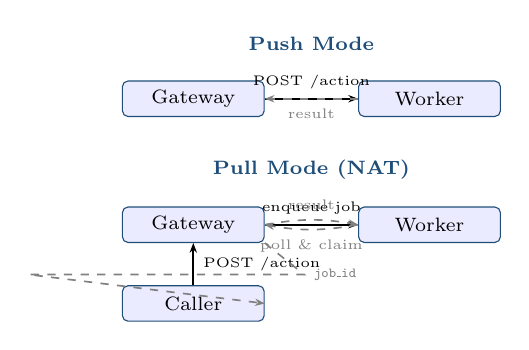
\begin{tikzpicture}[
  node distance=0.6cm,
  box/.style={draw, rounded corners=2pt, font=\scriptsize,
              fill=blue!8, draw=accentblue,
              minimum width=1.8cm, minimum height=0.45cm},
  arr/.style={-{Stealth[length=3.5pt]}, line width=0.6pt},
  darr/.style={-{Stealth[length=3.5pt]}, dashed, line width=0.6pt, gray},
  lbl/.style={font=\tiny, above, midway},
  lblb/.style={font=\tiny, below, midway},
]

% PUSH MODE
\node[font=\scriptsize\bfseries, color=accentblue] at (0, 0.1) {Push Mode};
\node[box] (gw1) at (-1.5,-0.6) {Gateway};
\node[box] (w1)  at (1.5,-0.6)  {Worker};
\draw[arr] (gw1) -- node[lbl]{POST /action} (w1);
\draw[darr] (w1) -- node[lblb]{result} (gw1);

% PULL MODE
\node[font=\scriptsize\bfseries, color=accentblue] at (0, -1.5) {Pull Mode (NAT)};
\node[box] (gw2)    at (-1.5,-2.2) {Gateway};
\node[box] (caller) at (-1.5,-3.2) {Caller};
\node[box] (w2)     at (1.5,-2.2)  {Worker};

\draw[arr] (caller.north) -- node[right, font=\tiny]{POST /action} (gw2.south);
\draw[arr] (gw2.east) -- node[lbl]{enqueue job} (w2.west);
\draw[darr] (gw2.south east) -- ++(0.5,-0.4) node[right, font=\tiny]{\texttt{job\_id}} -- ++(-3.5,0) -- (caller.east);
\draw[darr, bend left=10] (w2.west) to node[lblb]{poll \& claim} (gw2.east);
\draw[darr, bend left=10] (gw2.east) to node[lbl]{result} (w2.west |- gw2.east);

\end{tikzpicture}
\caption{Push mode (direct proxy) vs.\ pull mode (queue-based) delivery.}
\label{fig:pushpull}
\end{figure}

\textbf{Claim atomicity.} Multiple worker replicas polling concurrently
are safe: job claiming is protected by an asyncio lock, and only the
first \texttt{POST /jobs/\{job\_id\}/claim} succeeds.

\textbf{Pull job timeout.} Jobs that remain unclaimed beyond
\texttt{pull\_job\_timeout\_seconds} are marked \texttt{failed} lazily
at \texttt{GET /result} query time---consistent with the system-wide
lazy evaluation principle described in Section~\ref{sec:lazy}.

\subsection{Lazy Evaluation Pattern}
\label{sec:lazy}

A recurring design choice in GNOT is \emph{lazy evaluation}: rather than
maintaining background processes to sweep for stale state, GNOT applies
state checks at the moment the state is consulted. This pattern is
applied uniformly to:

\begin{itemize}[noitemsep, leftmargin=12pt]
  \item \textbf{Node staleness:} A node's heartbeat age is checked at
    routing time, not by a background timer.
  \item \textbf{Pull job timeout:} Checked at \texttt{GET /result} time,
    not by a background cleanup loop.
  \item \textbf{Upload TTL:} Expired files are removed on listing and on
    \texttt{GET /download}, not by a background sweeper.
  \item \textbf{Session expiry:} Sessions are silently recreated at
    \texttt{get\_or\_create()} time if expired.
\end{itemize}

Lazy evaluation eliminates background task coordination overhead, makes
behavior deterministic and testable, and ensures that routing decisions
are made with information current at the moment they matter.

\section{LLM Control Plane}
\label{sec:agent}

\subsection{LLM Provider Configuration}

\texttt{POST /intent} is available only on nodes that have an LLM
provider configured in \texttt{node.yaml}. GNOT supports any
OpenAI-compatible API as a provider, covering a wide range of
deployment scenarios:

\begin{lstlisting}[caption={LLM provider configuration examples}]
# External API (Anthropic Claude)
llm_provider: anthropic
llm_model: claude-sonnet-4-5
llm_api_key: sk-ant-...

# External API (OpenAI)
llm_provider: openai
llm_model: gpt-4o
llm_api_key: sk-...

# Local inference (Ollama)
llm_provider: ollama
llm_model: llama3.1:8b
llm_base_url: http://localhost:11434/v1

# Local inference (vLLM, LM Studio, etc.)
llm_provider: openai_compatible
llm_model: mistral-7b-instruct
llm_base_url: http://localhost:8000/v1
\end{lstlisting}

A node with no \texttt{llm\_provider} configured is a pure execution
node: it exposes \texttt{POST /action} only and incurs zero inference
cost. This makes GNOT deployable on resource-constrained edge machines
that cannot run or afford LLM inference, while still participating
fully in the mesh as action executors (see Section~\ref{sec:dual}).

\subsection{Intent Handling and ReAct Loop}

\texttt{POST /intent} is the primary human-facing endpoint. It accepts a
free-text prompt and executes a ReAct loop internally:

\begin{lstlisting}[caption={ReAct loop pseudocode}]
handle(request):
  session = get_or_create(session_id)
  session.add("user", prompt)
  system_prompt = build_from_live_capability_tree()

  for turn in range(max_turns):
    response = llm.chat(session.messages,
                         tools=[MESH_TOOL],
                         temperature=0.2)
    if response.tool_calls:
      for call in response.tool_calls:
        result = router.route(ActionRequest(call))
        if async: poll until complete
        session.add_tool_result(result)
      continue   // next turn
    else:
      return IntentResponse(reply=response.text)

  return IntentResponse(truncated=True)
\end{lstlisting}

The loop terminates when the LLM produces a plain-text response (no tool
calls) or when \texttt{max\_turns} is reached.

\subsection{Single Generic Tool Design}

A key design decision is exposing a single \texttt{mesh\_action} tool
to the LLM rather than one tool per action per node:

\begin{lstlisting}[language=, caption={The mesh\_action tool schema}]
{
  "name": "mesh_action",
  "parameters": {
    "target_node_id": "string",
    "action":         "string",
    "params":         "object"
  }
}
\end{lstlisting}

This design has two important properties. First, the tool registration
is \emph{stable}: new nodes and new actions join the mesh without
modifying the tool schema. Second, the LLM acquires capability knowledge
from the dynamically generated system prompt rather than from static
tool definitions, keeping the tool interface minimal.

\subsection{Dynamic System Prompt}

The \texttt{IntentHandler} builds the system prompt from the live
capability tree at each request, including node liveness status:

\begin{lstlisting}[caption={Excerpt of generated system prompt}]
## Mesh topology
- deb-0 [gateway, THIS NODE]
  - execute_command: Execute shell command
  - read_file, write_file

- cen-0 (direct, online)
  - execute_command, read_file, write_file

- cfsnk-0a via cfsnk-0 (online)
  - get_order_info: Retrieve CRM order details
    param order_id (string, required)
    [CREDENTIAL REQUIRED] crm_user_token

- cfsnk-0b via cfsnk-0 [UNREACHABLE]
  - send_notification: ...
\end{lstlisting}

Nodes marked \texttt{[UNREACHABLE]} are excluded from routing; the LLM
does not attempt to call them, avoiding multi-minute timeout waits.

\subsection{Session Management}

Sessions are identified by a caller-supplied \texttt{session\_id}
(e.g., a Telegram \texttt{chat\_id} or UUID). The
\texttt{ConversationStore} maintains the full OpenAI-format message
history across multiple \texttt{POST /intent} calls, enabling stateful
multi-turn conversations. Sessions expire after a configurable TTL;
expiry is checked lazily at session access time.

\section{Action Model}
\label{sec:actions}

\subsection{Seed Actions}

Three primitive actions constitute the bootstrap kernel and are present
on every node:

\begin{itemize}[noitemsep, leftmargin=12pt]
  \item \texttt{execute\_command}: Executes an arbitrary shell command
    and returns \texttt{stdout}, \texttt{stderr}, and \texttt{exit\_code}.
    This is the most powerful primitive: it enables installing software,
    writing configurations, starting processes, and bootstrapping new
    GNOT nodes.
  \item \texttt{read\_file}: Reads and returns the text content of a
    file at a specified path.
  \item \texttt{write\_file}: Writes text content to a file, creating
    parent directories as needed.
\end{itemize}

\subsection{Plugin Action Contract}

Custom actions are Python modules placed in a node's \texttt{actions/}
directory. The runtime loads them at startup via the following contract:

\begin{lstlisting}[language=python, caption={Plugin action contract}]
# Synchronous action
def run(params: dict, context: dict) -> dict: ...

# Asynchronous action
ASYNC = True
async def run(params: dict, context: dict) -> dict: ...
\end{lstlisting}

The \texttt{context} dict is injected by the runtime and includes:
\texttt{task\_id}, \texttt{job\_id}, \texttt{node\_id}, the full
\texttt{NodeConfig}, a shared \texttt{LLMClient}, a temporary directory
path, and \texttt{caller\_credentials}.

\subsection{JSON Schema Validation and Discovery}

Each action may have a co-located \texttt{\{action\}.schema.json} file
(JSON Schema Draft 7). Schemas serve three purposes: (1) request
validation before execution, returning HTTP 422 on failure; (2) LLM
guidance via the \texttt{GET /capabilities} endpoint and system prompt;
(3) caller credential declaration via the \texttt{x-caller-credentials}
vendor extension.

\section{Security Model}
\label{sec:security}

\subsection{Authentication Layers}

GNOT implements security at two layers:

\textbf{HTTP layer (AuthMiddleware).} Every non-exempt endpoint requires
a Bearer token. GNOT v5.13 introduced a per-node token model: the
gateway maintains an \texttt{allowed\_tokens} list, and each worker has
a unique token. This enables single-node revocation without
cluster-wide rotation. Token comparison uses \texttt{secrets.compare\_digest}
(constant-time) to prevent timing attacks.

\textbf{Action layer (CallerPolicies).} Individual actions can be
further restricted per-caller-token via \texttt{caller\_policies} in
\texttt{node.yaml}:

\begin{lstlisting}[caption={Action-level authorization example}]
caller_policies:
  - token: "sk-sales-team"
    allowed_actions: [get_order_info, list_orders]
  - token: "sk-devops"
    allowed_actions: [execute_command, read_file]
  - token: "sk-admin"
    allowed_actions: "*"
\end{lstlisting}

\subsection{Caller Credential System}

Some actions require credentials that the \emph{caller} supplies---for
example, a CRM API token that the calling user must own. These are
distinct from service credentials (database passwords, etc.) managed by
the action internally.

Caller credentials are transported in the \texttt{caller\_credentials}
field of \texttt{ActionRequest}, propagated through the full push/pull
chain, injected into action context, and \emph{never logged, never
stored in params, never appear in response bodies}.

\subsection{AES-256-GCM Credential Storage}

For multi-turn sessions via \texttt{POST /intent}, the
\texttt{CredentialStore} allows a caller to supply credentials once and
reuse them across subsequent turns. Credentials are stored encrypted
using AES-256-GCM with per-session key derivation:

\begin{equation}
k_{\text{session}} = \text{SHA-256}(\texttt{enc\_key} \;\|\; \texttt{:} \;\|\; \texttt{session\_id})
\label{eq:keyderivation}
\end{equation}

Per-session key derivation (Eq.~\ref{eq:keyderivation}) ensures that
compromising one session's key does not affect other sessions. The
encryption key (\texttt{credential\_encryption\_key}) is separate from
the authentication token (\texttt{auth\_token}), allowing each to be
rotated independently.

Persistence uses a write-through pattern with atomic file rename:
credentials are written to a \texttt{.tmp} file and atomically renamed
to the target path, ensuring readers never observe a partial write.

\section{Self-Bootstrapping}
\label{sec:bootstrap}

\subsection{Seed-to-Mesh Bootstrap}

The three seed actions are sufficient to create any new GNOT node. The
LLM orchestrates the following sequence via sequential \texttt{mesh\_action}
tool calls:

\begin{lstlisting}[caption={LLM-orchestrated node bootstrap sequence}]
1. execute_command: "mkdir -p /opt/mesh/node-B/actions"
2. write_file: path=/opt/mesh/node-B/node.yaml
               content=<generated node config>
3. write_file: path=.../actions/custom.py
               content=<generated action code>
4. execute_command: "pip install <deps>"
5. execute_command: "nohup python node_runtime.py \
                     --config node-B/node.yaml &"
6. execute_command: "curl -sf localhost:8081/health"
\end{lstlisting}

No external provisioning tool, configuration management system, or
container orchestrator is required. The LLM \emph{is} the provisioning
layer.

\subsection{One-Liner Worker Enrollment}

Any Linux machine can join the mesh with a single command:

\begin{lstlisting}[language=bash]
curl -sSL https://gateway.example.com/setup.sh \
  | bash -s -- --node-id cen-0 \
               --auth-token "$TOKEN" \
               --systemd
\end{lstlisting}

\texttt{GET /setup.sh} returns a universal setup script (auto-injected
with the gateway URL). The script handles OS detection (Debian/Ubuntu,
CentOS/RHEL, AlmaLinux, Arch, Alpine), Python 3.10+ installation,
virtualenv creation, runtime download, \texttt{node.yaml} generation,
and systemd service creation. Both \texttt{/setup.sh} and
\texttt{/runtime-bundle} are authentication-exempt so they can be
fetched before a token is available.

\subsection{Evolution Levels}

GNOT clusters evolve through four levels:

\begin{table}[h]
\centering
\caption{Cluster evolution levels}
\label{tab:evolution}
\small
\begin{tabular}{@{}clp{4.0cm}@{}}
\toprule
\textbf{Level} & \textbf{State} & \textbf{Description} \\
\midrule
L0 & Seed Only & Single node, 3 actions \\
L1 & Functional Nodes & Domain-specific nodes (DB, API, ML) \\
L2 & Specialized Clusters & GPU, storage, CPU-heavy workers \\
L3 & Self-Optimization & LLM replaces slow nodes, scales on queue depth \\
\bottomrule
\end{tabular}
\end{table}

At L3, the LLM can autonomously decide to bootstrap additional worker
nodes when it observes growing queue depth in \texttt{GET /health}'s
\texttt{queue\_depths} field, then decommission them when load subsides.

\section{File Transfer System}
\label{sec:files}

The seed action \texttt{write\_file} writes content inline in a JSON
payload, practical for text files up to approximately 1~MB. For binary
files (database dumps, compressed archives) at hundreds of megabytes,
GNOT provides a dedicated staged transfer mechanism.

The gateway's \texttt{UploadManager} accepts \texttt{multipart/form-data}
uploads and returns a \texttt{file\_id}. Workers on separate NAT layers
can then pull the file via \texttt{GET /download/\{file\_id\}}:

\begin{lstlisting}[language=bash, caption={Cross-NAT binary file transfer}]
# Step 1: Worker cen-0 uploads backup to gateway
curl -X POST https://gw/upload \
  -H "Authorization: Bearer $TOKEN" \
  -F "file=@/tmp/backup.sql.gz"
# => { "file_id": "a3f9b2c1d4e5f678" }

# Step 2: Worker alm-0 downloads from gateway
curl -OJ https://gw/download/a3f9b2c1d4e5f678 \
  -H "Authorization: Bearer $TOKEN"
\end{lstlisting}

This mechanism enables complete workflows such as cross-NAT database
migration orchestrated by a single \texttt{POST /intent}.

\section{Production Deployment}
\label{sec:deployment}

GNOT has been deployed in a production environment. The reference cluster
comprises four heterogeneous Linux nodes:

\begin{table}[h]
\centering
\caption{Reference production cluster}
\label{tab:cluster}
\small
\begin{tabular}{@{}lllp{2.8cm}@{}}
\toprule
\textbf{Node} & \textbf{OS} & \textbf{Mode} & \textbf{Connectivity} \\
\midrule
deb-0 & Debian & Gateway & Public via Cloudflare Tunnel \\
cen-0 & CentOS & Worker & Private, pull-only \\
alm-0 & AlmaLinux & Worker & Private, pull-only \\
cfsnk-0 & CentOS & Worker & Private, pull-only \\
\bottomrule
\end{tabular}
\end{table}

All three workers operate behind NAT and are therefore pull-only: they
never receive inbound connections. The gateway is exposed via a
Cloudflare Tunnel, requiring no port forwarding or public IP on the
host machine. Workers make outbound HTTPS connections to the gateway
exclusively.

\subsection{Production Use Cases}

The following four use cases have been validated on the production
cluster. Each is initiated by a single natural-language prompt with
zero pre-written workflow code. They are presented in order of
increasing architectural complexity.

\subsubsection{Cross-Network Database Migration}

Two worker nodes (\texttt{cen-0} and \texttt{cfsnk-0}) reside on
separate private networks with no direct connectivity. A MySQL database
hosted on \texttt{cfsnk-0} must be migrated to \texttt{cen-0}.

The LLM orchestrates the following sequence entirely through the mesh:

\begin{enumerate}[noitemsep, leftmargin=14pt]
  \item \texttt{execute\_command} on \texttt{cfsnk-0}: \texttt{mysqldump
    > /tmp/db.sql.gz} — exports and compresses the database.
  \item \texttt{POST /upload} to gateway (\texttt{deb-0}): transfers
    the dump file via the staged binary upload mechanism.
  \item \texttt{GET /download/\{file\_id\}} from \texttt{cen-0}:
    worker pulls the dump from the gateway.
  \item \texttt{execute\_command} on \texttt{cen-0}: restores the dump
    into the target MySQL instance.
\end{enumerate}

This workflow crosses two NAT boundaries (\texttt{cfsnk-0}
$\to$ gateway $\to$ \texttt{cen-0}) without any direct tunnel or VPN
between the two machines. The \texttt{UploadManager}'s staged transfer
(Section~\ref{sec:files}) acts as the data relay point.

\subsubsection{Telegram-Based Order Tracking}

A customer-facing Telegram bot is integrated with an internal CRM
system running on a private network node (\texttt{cfsnk-0a}). The
gateway node (\texttt{deb-0}) runs both the Telegram webhook handler
and the \texttt{IntentHandler}.

When a customer sends an order number via Telegram, the bot forwards
the message as a \texttt{POST /intent} request to the gateway. The
LLM resolves the intent, calls \texttt{get\_order\_info} on
\texttt{cfsnk-0a} via the pull-mode delivery chain, and returns the
result as a natural-language Telegram reply. The CRM node never
requires a public address; the pull-mode delivery model
(Section~\ref{sec:pushpull}) handles connectivity transparently.

The customer's CRM API token is supplied once per Telegram session
via \texttt{caller\_credentials} and stored encrypted in the
\texttt{CredentialStore} for the session duration, so subsequent
queries within the same session require no re-authentication.

\subsubsection{Autonomous Software Development}

A developer provides a natural-language feature description or bug
report via \texttt{POST /intent}. The LLM autonomously performs the
complete development cycle using only the three seed actions:

\begin{enumerate}[noitemsep, leftmargin=14pt]
  \item \texttt{read\_file} — inspects relevant source files and test
    suites in the target codebase.
  \item \texttt{write\_file} — writes new source files or applies
    targeted fixes to existing ones.
  \item \texttt{execute\_command} — runs the test suite
    (\texttt{python -m pytest}) and re-iterates if tests fail.
  \item \texttt{execute\_command} — deploys the change (restart
    service, run migration, or copy artifacts) on the same node or
    a designated deployment node.
\end{enumerate}

The LLM's ReAct loop handles test failures as observations: if
\texttt{pytest} returns a non-zero exit code, the LLM reads the
failure output, revises the implementation, and re-runs tests---all
within the same \texttt{POST /intent} turn sequence, without any
human intervention. Both greenfield feature development and bug
fixing have been validated with this approach.

\subsubsection{Automated YouTube Content Pipeline}

A content creator provides a topic as a single natural-language prompt.
The LLM orchestrates a complete content production and publishing
pipeline across mesh nodes:

\begin{enumerate}[noitemsep, leftmargin=14pt]
  \item \textbf{Research:} \texttt{execute\_command} invokes a web
    search or summarization script to gather topic material.
  \item \textbf{Script generation:} The LLM generates a narration
    script, which \texttt{write\_file} saves to the working node.
  \item \textbf{Media generation:} \texttt{execute\_command} calls
    an AI image/video generation API (e.g., Stable Diffusion,
    text-to-video model) to produce visual assets for each segment.
  \item \textbf{Video rendering:} \texttt{execute\_command} invokes
    \texttt{ffmpeg} to assemble narration audio (TTS) and visual
    assets into a final video file.
  \item \textbf{Upload:} \texttt{execute\_command} calls the YouTube
    Data API v3 to upload the rendered video with generated title,
    description, and tags.
\end{enumerate}

This use case demonstrates that GNOT's orchestration model extends
naturally to creative and media workflows. The entire pipeline---from
topic input to published video---runs without the creator writing or
executing any code. The mesh nodes provide the compute; the LLM
provides the workflow logic.

\subsubsection{Summary}

Table~\ref{tab:usecases} summarizes the four use cases by the
architectural features they exercise.

\begin{table}[h]
\centering
\caption{Production use cases and architectural features exercised}
\label{tab:usecases}
\small
\begin{tabular}{@{}lcccc@{}}
\toprule
\textbf{Feature} &
  \rotatebox{60}{\textbf{DB Migrate}} &
  \rotatebox{60}{\textbf{Telegram CRM}} &
  \rotatebox{60}{\textbf{Auto Coding}} &
  \rotatebox{60}{\textbf{YouTube}} \\
\midrule
Cross-NAT delivery      & \checkmark & \checkmark &            &            \\
Pull-mode workers       & \checkmark & \checkmark & \checkmark & \checkmark \\
Binary file transfer    & \checkmark &            &            & \checkmark \\
Caller credentials      &            & \checkmark &            &            \\
Multi-turn ReAct loop   &            &            & \checkmark & \checkmark \\
External API calls      &            &            &            & \checkmark \\
Session persistence     &            & \checkmark &            &            \\
Seed actions only       & \checkmark &            & \checkmark & \checkmark \\
\bottomrule
\end{tabular}
\end{table}

No use case required any pre-written workflow code, DAG definition, or
configuration beyond the standard \texttt{node.yaml}. All orchestration
logic was generated at runtime by the LLM from a single natural-language
prompt.

\section{Discussion}
\label{sec:discussion}

\subsection{Design Decisions}

\textbf{D1: Why lazy evaluation over background polling?}
Background staleness detection requires coordination between the
detection task and the routing path. Lazy evaluation removes this
coordination entirely: state is always consistent at the moment it is
read, and the system has one fewer category of concurrency bug.

\textbf{D2: Why the BGP analogy?}
BGP solves an analogous problem at internet scale: enabling arbitrary
routers to reach arbitrary destinations without knowing full paths. The
key insight---that routers need only know the \emph{next hop}, not the
full path---maps cleanly to GNOT's requirement that the gateway need
only know which intermediate node to forward to, not the full path to
the target.

\textbf{D3: Why a single \texttt{mesh\_action} tool?}
Per-action tools would require the tool registration to be updated
whenever the mesh topology changes. A single generic tool with a stable
schema decouples the tool interface from the capability surface,
allowing the mesh to grow dynamically without LLM re-prompting overhead.

\textbf{D4: Why AES-256-GCM over a KMS?}
KMS integration introduces deployment dependencies (IAM roles, network
policies, service availability) incompatible with GNOT's design goal of
minimal operational footprint. AES-256-GCM with per-session key
derivation provides strong isolation at the cost of a single symmetric
secret.

\textbf{D5: Why separate \texttt{credential\_encryption\_key} from
\texttt{auth\_token}?}
Security best practice requires rotating authentication tokens
periodically. Without separation, token rotation would invalidate all
active sessions---a non-obvious side effect. Separating the two keys
allows each to be rotated on its own schedule.

\textbf{D6: Why per-node tokens rather than a shared cluster token?}
A shared cluster token means revoking a compromised worker requires a
cluster-wide rotation, temporarily disrupting all nodes. Per-node tokens
allow the gateway to revoke a single worker by removing its token from
\texttt{allowed\_tokens}, leaving all other nodes unaffected. The
implementation overhead is minimal: token validation is a frozenset
membership lookup per request.

\subsection{Limitations}

The current implementation has three known limitations of architectural
significance:

\begin{itemize}[noitemsep, leftmargin=12pt]
  \item \textbf{No container isolation.} \texttt{execute\_command} has
    full host filesystem access. The intended mitigation is to run each
    node as a dedicated non-root OS user with restricted permissions.
    Container-level isolation via Docker or nsjail would require
    careful integration to avoid breaking the seed bootstrapping
    sequence, which itself uses \texttt{execute\_command} to install
    software and start processes.

  \item \textbf{In-memory pull queue.} The \texttt{JobQueue} is held
    in process memory. A gateway restart loses all undelivered queued
    jobs. The configurable \texttt{pull\_job\_timeout\_seconds} bounds
    the exposure window for any individual job, but jobs enqueued
    immediately before a restart are silently dropped. A SQLite-backed
    durable queue is planned.

  \item \textbf{Hot-reload configuration.} Adding or revoking tokens
    in \texttt{node.yaml} requires a node restart to take effect.
    \texttt{AuthMiddleware} loads the \texttt{allowed\_tokens}
    frozenset once at startup. A SIGHUP handler or inotify watch on
    \texttt{node.yaml} would resolve this without downtime.
\end{itemize}

\subsection{Future Work}

Table~\ref{tab:futurework} lists planned improvements by priority.

\begin{table}[h]
\centering
\caption{Planned improvements}
\label{tab:futurework}
\small
\begin{tabular}{@{}clp{4.2cm}@{}}
\toprule
\textbf{Pri.} & \textbf{Feature} & \textbf{Description} \\
\midrule
P1 & SSE streaming & \texttt{POST /intent} returns \texttt{text/event-stream} with turn-by-turn updates \\
P1 & Durable job queue & SQLite-backed \texttt{JobQueue} surviving gateway restarts \\
P2 & Hot-reload config & SIGHUP or inotify watch on \texttt{node.yaml} for token changes \\
P2 & Token audit logging & Map token fingerprint → node identity in access logs \\
P3 & Container isolation & Optionally run actions in Docker or nsjail per node \\
P3 & Metrics endpoint & Prometheus \texttt{/metrics}: job throughput, queue depths, latency \\
P3 & Topology dashboard & Read-only web UI for mesh topology and job history \\
\bottomrule
\end{tabular}
\end{table}

The multi-network membership model (one node joining multiple gateways),
event emit/subscribe between nodes, and a built-in scheduler for
periodic action invocation are planned as the primary architectural
extensions in GNOT v2.

\textbf{Evolution context.} GNOT reached its current architecture
through 14 incremental versions (v5.0--v5.13b). Each version added
one well-scoped capability: v5.3 introduced push/pull delivery, v5.7
added lazy staleness detection, v5.9 added the \texttt{POST /intent}
ReAct loop, v5.10 added BGP-style route advertisement, v5.12 added
AES-256-GCM credential encryption, and v5.13b introduced the per-node
token model. This incremental approach ensured each mechanism could be
validated independently before the next layer was added.

\section{Conclusion}
\label{sec:conclusion}

We have presented GNOT, a distributed execution mesh architected for
native LLM orchestration. Rather than wrapping infrastructure in
LLM-specific tool SDKs, GNOT exposes a uniform, self-describing
interface---\texttt{POST /action}, \texttt{GET /capabilities}, and a
single \texttt{mesh\_action} tool schema---that any tool-calling-capable
LLM can operate without framework integration or pre-written workflow
code.

The key architectural contributions---minimal-seed bootstrap,
BGP-inspired NAT traversal, transparent push/pull delivery, lazy
evaluation, and per-session AES-256-GCM credentials---combine into a
coherent system that is simultaneously simple to deploy (a single Python
process per node) and capable of coordinating complex workflows across
machines that have never been directly connected.

Production experience with the reference four-node cluster demonstrates
that using a frontier model---Claude, accessed via its web
interface---as the external orchestrator yields strong practical results:
the full capability surface of a continuously improving model is
available at subscription cost, with zero inference overhead on any mesh
node. The four validated use cases (cross-network database migration,
Telegram CRM integration, autonomous software development, and automated
content publishing) were each accomplished through a single
natural-language prompt with no pre-written workflow code.

We release the reference implementation at
\url{https://github.com/gnot-io/gnot}~\cite{gnot2026} under the Apache
2.0 license and invite the research community to explore the broader
space of LLM-native distributed infrastructure.

\section*{Acknowledgments}

The author thanks the open-source communities behind FastAPI, Pydantic,
httpx, and the broader Python async ecosystem, without which this
implementation would not have been feasible at the present scale.

% ── References ────────────────────────────────────────────────────────────
\begin{thebibliography}{9}

\bibitem{langchain2023}
  Chase, H. (2022).
  \textit{LangChain: Building applications with LLMs through composability}.
  \url{https://github.com/langchain-ai/langchain}

\bibitem{react2022}
  Yao, S., Zhao, J., Yu, D., Du, N., Shafran, I., Narasimhan, K., and
  Cao, Y. (2022).
  ReAct: Synergizing Reasoning and Acting in Language Models.
  \textit{arXiv preprint arXiv:2210.03629}.
  \url{https://arxiv.org/abs/2210.03629}

\bibitem{rekhter1995bgp}
  Rekhter, Y. and Li, T. (1995).
  A Border Gateway Protocol 4 (BGP-4).
  \textit{RFC 1771}, Internet Engineering Task Force.
  \url{https://www.rfc-editor.org/rfc/rfc1771}

\bibitem{gnot2026}
  Tran, V. (2026).
  \textit{GNOT: Generative Node Orchestration Technology --- Reference
  Implementation v5.13}.
  gnot-io/gnot, GitHub.
  \url{https://github.com/gnot-io/gnot}
  Apache License 2.0.

\end{thebibliography}

\end{document}
